\documentclass[10pt]{article}

\usepackage[margin=1in]{geometry}
\usepackage{booktabs}
\usepackage{graphicx}
\usepackage{microtype}
\usepackage{url}
\usepackage[hidelinks]{hyperref}

\graphicspath{{figures/}}

\newcommand{\code}[1]{\texttt{#1}}

\title{Speculative Decoding for Hybrid SSM--Attention Models:\\
A Case Study with PLaMo 2 on llama.cpp}
\author{Gurunath Lunkupali Venugopal}
\date{June 2026}

\begin{document}

\maketitle

\begin{abstract}
Speculative decoding is a standard technique for accelerating autoregressive
LLM inference, but it is poorly supported for hybrid state-space-model (SSM)
architectures: the fixed-size recurrent state of Mamba-style layers cannot be
truncated on token rejection the way a KV cache can. This was long a
practical blocker---as recently as late 2025, vLLM rejected all
speculative-decoding methods on Mamba-hybrid models outright---but by mid-2026
the rollback problem had been solved generically across several stacks
(llama.cpp, and conditionally vLLM and SGLang), which independently converged
on the same snapshot-and-restore primitive (Section~\ref{sec:discussion}).
\textbf{We run our experiment on llama.cpp on a single laptop} (Apple
M4~Pro, Metal backend, build b9596) and do not benchmark the other engines.
We measure \code{pfnet/plamo-2-8b} (target) with \code{pfnet/plamo-2-1b}
(draft) across three task families with greedy sampling, verifying
byte-identical outputs versus the non-speculative baseline. The result is a carefully measured
\emph{negative} one: despite token acceptance rates up to 90\% and a draft
model that is $6.3\times$ faster standalone, draft-model speculation is
never profitable on this hardware (best case $0.99\times$; worst
$0.29\times$). Only model-free n-gram (prompt-lookup) drafting yields a
speedup, and only on translation ($1.21\times$). We attribute the slowdown
to per-round costs---serial draft decoding, batched verification, and
$\sim$33.5\,MiB SSM-state checkpoints---that exceed the savings on
bandwidth-bound consumer hardware. Along the way we discovered a novel
quantization bug: quantizing PLaMo~2's Mamba output projection
(\code{ssm\_out}) to Q8\_0 causes degenerate generation on
newline-containing prompts in both the 1B and 8B models; we isolate the
faulty tensor experimentally and provide a one-flag mitigation that likely
applies to all community PLaMo~2 GGUFs.
\end{abstract}

\section{Introduction \& Motivation}

PLaMo~2 is Preferred Networks' (PFN) family of Japanese/English foundation
models built on a Samba-style hybrid architecture that interleaves Mamba2
state-space (SSM) layers with sliding-window attention~\cite{plamo2tr}. Hybrid
SSM--attention models are attractive for inference because the SSM layers
replace an ever-growing KV cache with a fixed-size recurrent state, but that
same property breaks one of the most widely used inference accelerations:
speculative decoding.

Speculative decoding drafts $k$ candidate tokens cheaply (with a small draft
model, or model-free heuristics such as prompt lookup), verifies them in a
single batched forward pass of the target model, and---under greedy
sampling---is \emph{lossless}: output is provably identical to plain
decoding. The catch for hybrid models is rejection. With a pure transformer,
rejecting speculated tokens means truncating the KV cache, an $O(1)$
bookkeeping operation. With an SSM layer, the recurrent state after
processing $k$ tokens has irreversibly mixed those tokens in; there is no
truncation operator. This was historically a practical blocker: as recently
as late 2025, vLLM raised a \code{NotImplementedError} (``Mamba with
speculative decoding is not supported yet'') for \emph{all} speculative
methods on Mamba-hybrid models~\cite{vllmissue}. By the time of our
measurements (mid-2026) the problem had been solved generically---first in
llama.cpp via per-sequence rolling checkpoints of SSM
state~\cite{llamacpppr}, and subsequently in vLLM and SGLang, which converged
on the same primitive (we survey the full landscape in
Section~\ref{sec:discussion}).

\textbf{Our experiment uses llama.cpp on a local MacBook}; we did not
benchmark vLLM or SGLang. We chose it for a clean, accessible implementation
on Apple Silicon, to ask an empirical question that, to our knowledge, has
not been answered for PLaMo~2: \emph{does speculative decoding actually pay
off on a hybrid SSM--attention model, once correctness is solved?} We answer
it for the PLaMo~2 8B/1B pair, with a rigorous losslessness check, and report
an honest negative result with a mechanistic explanation. As a
secondary, first-class contribution, we document and root-cause a PLaMo~2
quantization bug that silently corrupts generation in standard Q8\_0 GGUFs.

\section{Background}

\subsection{Samba-style hybrid architecture}

PLaMo~2 follows the Samba recipe: blocks of Mamba2 SSM layers interleaved
with sliding-window attention layers~\cite{plamo2tr}. The SSM layers carry a
fixed-size recurrent state (convolution state plus SSM state) per sequence;
the attention layers keep a bounded sliding-window KV cache. This gives
near-constant memory during decode, at the cost of state that evolves
destructively token by token.

\subsection{KV truncation vs.\ SSM state rollback}

In a transformer, speculative verification that accepts $a < k$ drafted
tokens simply discards KV entries for positions beyond $a$. An SSM has no
analogous operation: its state is a lossy summary of the whole prefix, so
``forgetting'' the last $k-a$ tokens requires having saved an earlier copy
of the state. This is exactly why vLLM's speculative-decoding path
originally refused Mamba-hybrid models for every proposer type (n-gram,
draft model, EAGLE, Medusa, MTP)~\cite{vllmissue}.

\subsection{llama.cpp's recurrent checkpoint mechanism}

llama.cpp addressed this generically in its recurrent memory module:
\code{llama\_memory\_recurrent} maintains a rolling buffer of checkpoints
(depth 8 per sequence) of the SSM state tensors, saved at batch boundaries
and restored when speculation is rejected~\cite{llamacpppr}. Correctness
becomes architecture-agnostic, but the checkpoints are not free: for the
PLaMo~2 8B, server logs in our runs reported approximately 33.5\,MiB per
context checkpoint. Every speculation round therefore adds state-copy
traffic on top of draft decoding and batched verification---a cost model
that turns out to matter a great deal in Section~\ref{sec:discussion}.

\section{A Quantization Bug Found Along the Way}
\label{sec:bug}

Before any speculation numbers could be trusted, we hit a correctness bug
that we believe affects all community PLaMo~2 GGUFs and present as a
first-class contribution.

\paragraph{Symptom.} In the first benchmark run, every prompt containing a
bare newline (token 10, the reserved byte token \code{0x0A})---i.e.\ all
code and translation prompts---returned \emph{empty} content while
``generating'' 256 tokens at full speed. This occurred with both the 1B and
the 8B Q8\_0 models.

\paragraph{Root-cause chain.} Each step below is one controlled experiment:

\begin{enumerate}
  \item Requesting raw token IDs (\code{return\_tokens: true}) revealed
    that the model emits token 31, i.e.\
    \code{<|plamo:}\allowbreak\code{reserved:}\allowbreak\code{0x1F|>},
    indefinitely;
    reserved tokens render as empty text and are not end-of-generation, so
    decoding runs to the limit.
  \item Tokenizer round-trip via \code{/tokenize} + \code{/detokenize} is
    perfect, including indented code. Not a tokenizer bug.
  \item Full prompt token-ID comparison, HF transformers vs.\ llama.cpp:
    identical (modulo BOS; manually prepending BOS changed nothing).
  \item Ground truth via HF transformers on CPU in fp32 (this required
    pinning \code{transformers<4.58} \emph{and} writing pure-PyTorch shims
    for the \code{causal\_conv1d} and \code{mamba\_ssm} reference functions,
    since pfnet's modeling code's CPU fallback still calls those packages):
    the reference implementation generates correct code for the failing
    prompt. Hence a llama.cpp-side problem.
  \item Unquantized bf16 GGUF in llama.cpp: correct output. Hence a
    quantization problem, not an inference-kernel problem.
  \item Re-quantizing to Q8\_0 from bf16 with \code{llama-quantize}: still
    broken. Hence not a converter bug.
  \item Per-tensor isolation with \code{--tensor-type X=bf16}
    (Table~\ref{tab:isolation}): keeping \code{ssm\_out} alone in bf16 fixes
    generation; exempting any other tensor does not.
\end{enumerate}

\begin{table}[ht]
\centering
\caption{Per-tensor isolation: which single tensor kept in bf16 (all else
Q8\_0) repairs generation on newline-containing prompts.}
\label{tab:isolation}
\begin{tabular}{llc}
\toprule
Tensor(s) kept in bf16 & Role & Output \\
\midrule
token embeddings & embedding & broken \\
output & LM head & broken \\
all \code{ssm\_*} matrices & all Mamba projections & \textbf{fixed} \\
\code{ssm\_in} & Mamba input projection & broken \\
\code{ssm\_x} & Mamba $x$ projection & broken \\
\code{ssm\_dt} & Mamba $\Delta t$ projection & broken \\
\code{ssm\_out} & Mamba output projection & \textbf{fixed} \\
\bottomrule
\end{tabular}
\end{table}

\paragraph{Conclusion and mitigation.} Quantizing PLaMo~2's Mamba output
projection (\code{ssm\_out}) to Q8\_0 causes degenerate generation on
newline-containing prompts. The mitigation is one flag:

\begin{quote}
\code{llama-quantize --tensor-type ssm\_out=bf16 model-BF16.gguf
model-Q8fixed.gguf Q8\_0}
\end{quote}

\paragraph{Impact.} The bug reproduces on both the 1B and 8B models and is a
property of the standard Q8\_0 recipe, so it likely affects all community
PLaMo~2 GGUFs published to date. Reported upstream as
\href{https://github.com/ggml-org/llama.cpp/issues/24501}{ggml-org/llama.cpp\#24501};
a natural fix is to protect \code{ssm\_out} in llama.cpp's plamo2 quantization recipe. All benchmarks in
this paper use the repaired quantization (``Q8fixed'': Q8\_0 with
\code{ssm\_out} in bf16) for \emph{both} models.

\section{Methodology}

\paragraph{Hardware and build.} MacBook Pro with Apple M4~Pro, 48\,GB
unified memory, Metal backend. llama.cpp build b9596 (official release
binaries), served via \code{llama-server}.

\paragraph{Models and quantization.} Target: \code{pfnet/plamo-2-8b}.
Draft: \code{pfnet/plamo-2-1b}. Both converted to GGUF and quantized to
Q8\_0 with \code{ssm\_out} kept in bf16 (Section~\ref{sec:bug}). Standalone,
the draft decodes at 134\,tok/s vs.\ 21.4\,tok/s for the target---a
$6.3\times$ ratio that would normally make draft-model speculation
attractive.

\paragraph{Configurations.}
\begin{itemize}
  \item \code{fx\_baseline}: plain decoding, no speculation.
  \item \code{fx\_spec\_d\{2,4,8,16\}}: draft-model speculation
    (\code{--spec-type draft-simple}) with \code{draft-n-max} $= 2, 4, 8,
    16$ and \code{draft-n-min} $= 1$.
  \item \code{fx\_ngram}: model-free n-gram speculation
    (\code{--spec-type ngram-simple}, prompt lookup; no draft model).
\end{itemize}

\paragraph{Tasks and protocol.} Twelve prompts spanning three task families
---\code{ja\_chat}, \code{translation\_en\_ja}, and \code{code}---each run
3 times per configuration (\code{bench/prompts.json}). Greedy sampling
(temperature 0, top-$k$ 1), \code{n\_predict} 256. We record decode
throughput, drafted/accepted token counts, and a SHA-256 hash of the full
generated text per prompt.

\paragraph{Losslessness verification.} For every prompt, the SHA-256 of the
speculative output is compared against the baseline output. All speculative
configurations produced byte-identical greedy output to the baseline,
confirming that llama.cpp's SSM checkpoint/rollback is exact.

\section{Results}
\label{sec:results}

Table~\ref{tab:final} reports median decode throughput per task, speedup
versus baseline, and token acceptance rate. The headline: with a real draft
model, speculation never wins on this hardware. The best draft-model cell
is \code{fx\_spec\_d2} on translation at $0.99\times$ (break-even);
ja\_chat degrades to $0.29\times$ at depth 16. The only profitable
configuration anywhere is n-gram drafting on translation ($1.21\times$),
with \code{fx\_spec\_d4} on translation near-breakeven-positive at
$1.18\times$.

\begin{table}[ht]
\centering
\caption{Median decode throughput in tok/s (speedup vs.\ baseline)
[token acceptance rate]. Greedy sampling; all speculative outputs
byte-identical to baseline.}
\label{tab:final}
\small
\begin{tabular}{lccc}
\toprule
Config & code & ja\_chat & translation\_en\_ja \\
\midrule
\code{fx\_baseline}  & 19.7 (1.00$\times$)            & 21.6 (1.00$\times$)            & 15.7 (1.00$\times$) \\
\code{fx\_ngram}     & 18.1 (0.92$\times$) [19\%]     & 17.6 (0.81$\times$) [63\%]     & \textbf{19.0 (1.21$\times$) [23\%]} \\
\code{fx\_spec\_d2}  & 16.5 (0.84$\times$) [90\%]     & 13.8 (0.64$\times$) [80\%]     & 15.5 (0.99$\times$) [87\%] \\
\code{fx\_spec\_d4}  & 12.0 (0.61$\times$) [77\%]     & 10.2 (0.47$\times$) [55\%]     & 18.5 (1.18$\times$) [70\%] \\
\code{fx\_spec\_d8}  & 11.6 (0.59$\times$) [55\%]     & \phantom{0}7.9 (0.36$\times$) [32\%] & 11.1 (0.71$\times$) [48\%] \\
\code{fx\_spec\_d16} & 11.7 (0.59$\times$) [33\%]     & \phantom{0}6.2 (0.29$\times$) [17\%] & \phantom{0}9.3 (0.59$\times$) [29\%] \\
\bottomrule
\end{tabular}
\end{table}

Figure~\ref{fig:speedup} summarizes speedups per task and configuration;
Figure~\ref{fig:acceptance} shows acceptance rates, which decay sharply with
draft depth; Figure~\ref{fig:dist} shows full throughput distributions
across prompts and repeats; Figure~\ref{fig:accept-speed} relates
acceptance to realized speed, making the central paradox visible: 90\%
acceptance still loses.

\begin{figure}[ht]
\centering
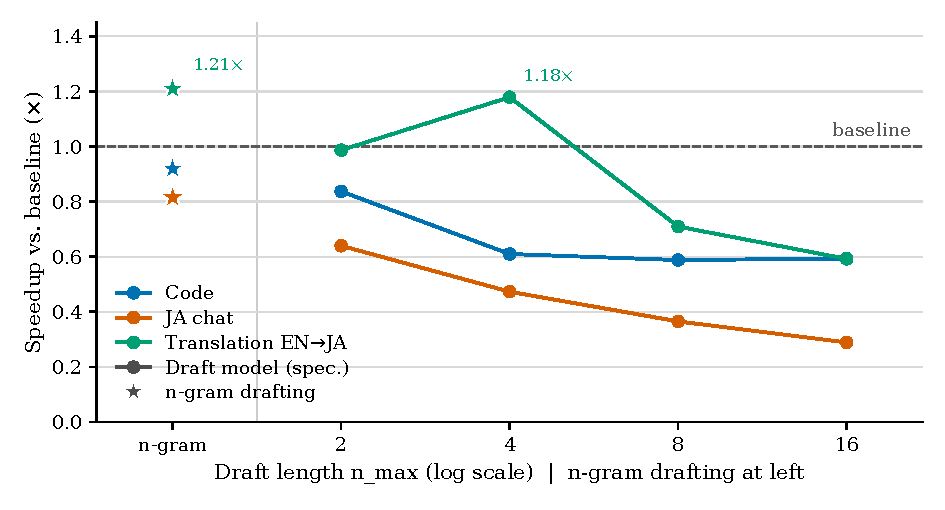
\includegraphics[width=0.85\textwidth]{fig1_speedup.pdf}
\caption{Decode speedup vs.\ baseline by task and configuration. Only
n-gram drafting on translation exceeds $1.0\times$; draft-model speculation
is unprofitable everywhere.}
\label{fig:speedup}
\end{figure}

\begin{figure}[ht]
\centering
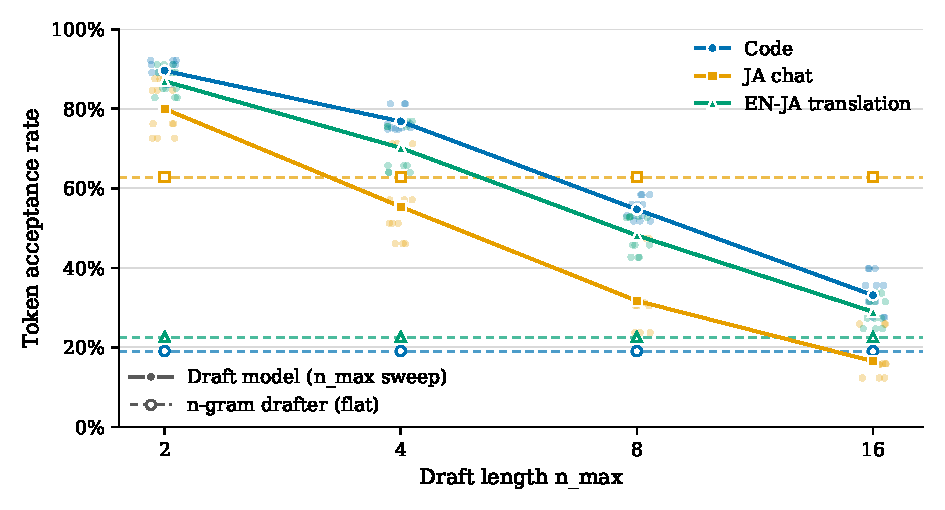
\includegraphics[width=0.85\textwidth]{fig2_acceptance.pdf}
\caption{Token acceptance rate by task and draft depth. Acceptance is
excellent at depth 2 (up to 90\%) but per-token acceptance decays with
depth, so deeper drafts amortize worse.}
\label{fig:acceptance}
\end{figure}

\begin{figure}[ht]
\centering
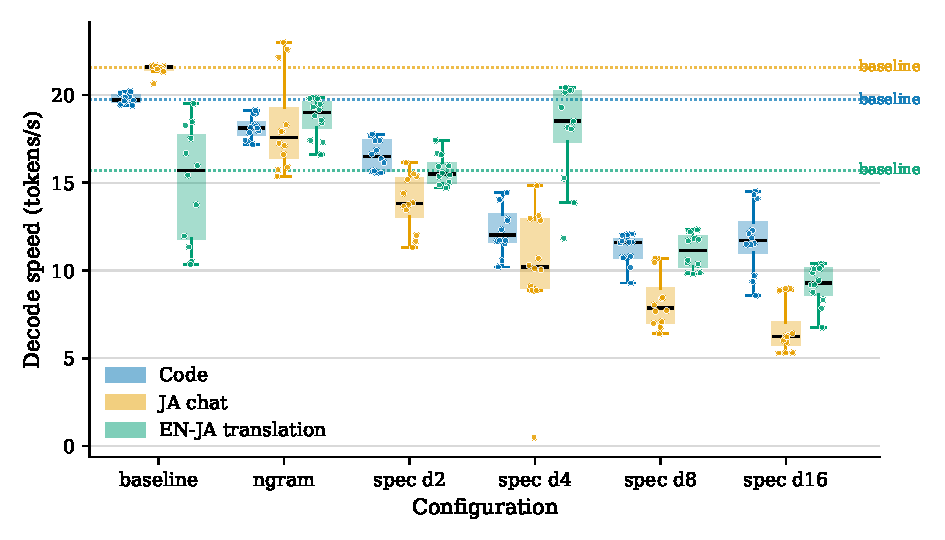
\includegraphics[width=0.85\textwidth]{fig3_distributions.pdf}
\caption{Decode throughput distributions across prompts and repeats for
each configuration and task.}
\label{fig:dist}
\end{figure}

\begin{figure}[ht]
\centering
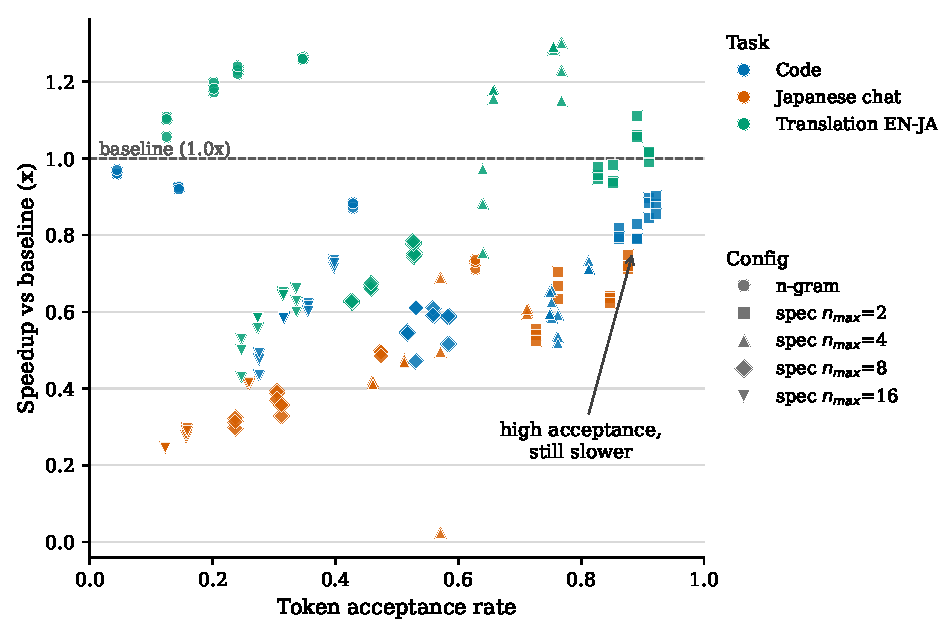
\includegraphics[width=0.85\textwidth]{fig4_acceptance_vs_speed.pdf}
\caption{Acceptance rate vs.\ realized decode speed. High acceptance does
not translate into speedup: per-round overheads dominate.}
\label{fig:accept-speed}
\end{figure}

\paragraph{Losslessness.} All speculative configurations produced
byte-identical greedy output to baseline, verified by SHA-256 per prompt.
The negative result is therefore purely about throughput, not correctness.

\section{Discussion}
\label{sec:discussion}

\paragraph{Why 90\% acceptance still loses.} Each speculation round pays
three costs that plain decoding does not: (i) \emph{serial draft-model
decode}---the 1B draft, though $6.3\times$ faster standalone, still runs
serially before each verification and competes for the same unified-memory
bandwidth; (ii) \emph{batched verification} in the target, which on
bandwidth-bound Metal hardware is far from free relative to single-token
decode (single-token decode already saturates memory bandwidth, so a
$k$-token verify costs nearly as much per token as plain decode); and (iii)
\emph{SSM-state checkpointing}---roughly 33.5\,MiB saved per context
checkpoint for the 8B, plus restores on rejection. At depth 2 with 90\%
acceptance (code), these round costs already eat the entire benefit
($0.84\times$). Deeper drafts amortize per-round costs over more tokens in
principle, but per-token acceptance decays with depth
(Figure~\ref{fig:acceptance}), so realized acceptance lengths grow slowly
while rejected work and rollbacks grow quickly: depth 16 lands at
$0.29$--$0.59\times$.

\paragraph{Why n-gram wins on translation.} Prompt-lookup drafting has
essentially zero proposal cost---no draft forward pass, no second model
resident in memory. Translation outputs copy long spans from the source
prompt verbatim (names, numbers, code-switched terms), so even a modest
23\% acceptance converts into free accepted tokens, yielding the study's
only speedup ($1.21\times$). On code, ja\_chat, and any task where output
text is not substring-recoverable from the prompt, lookup proposals miss
and the verification overhead makes it a net loss.

\paragraph{Implications.} These numbers temper the urgency that was, at the
time of writing, attached to lifting vLLM's Mamba-hybrid
speculative-decoding restriction~\cite{vllmissue}:
correctness machinery (as llama.cpp shows) is solvable, but a separate
draft model may simply not pay on bandwidth-bound hardware, and the
checkpoint traffic is an architecture-intrinsic tax. Cheap proposers
(n-gram, and especially self-drafting methods such as MTP or EAGLE-style
heads that reuse the target's hidden states and add no second model) are
the more promising direction for hybrids, since they attack the dominant
cost---the serial draft---directly. Notably, PLaMo~3 NICT models move to an
attention-only architecture, which sidesteps SSM rollback entirely and
restores cheap KV truncation; speculative decoding economics there should
look conventional again.

\paragraph{Framing.} We deliberately report this as a measured negative
result with a mechanism. ``Speculation is lossless and works, but is
unprofitable for PLaMo~2 8B/1B on M4~Pro Metal'' is directly actionable for
anyone deploying these models locally: run the baseline, or n-gram for
translation-like workloads.

\paragraph{Platform landscape and scope.} We benchmarked llama.cpp on a
single laptop and did not test other engines---a deliberate scope choice, not
a claim that llama.cpp is unique. As of our measurements (mid-2026), the
SSM-rollback problem had been solved in at least three stacks, which
independently converged on the same snapshot-and-restore primitive:
\begin{itemize}
  \item \textbf{llama.cpp} merged it as PR~\#19493~\cite{llamacpppr} (an
    earlier alternative, \#20075, was closed unmerged): the
    \code{llama\_memory\_recurrent} rolling checkpoint buffer used here.
  \item \textbf{vLLM}, which into early 2026 rejected the combination outright
    (\#30114~\cite{vllmissue}, closed April 2026), added it in
    PR~\#33726~\cite{vllmpr} (merged Feb 2026) and now supports it
    \emph{conditionally}---with \code{--mamba-cache-mode align} plus
    self-drafting heads such as EAGLE3 or MTP---though model-free n-gram
    drafting can still corrupt recurrent state on some hybrids.
  \item \textbf{SGLang} added it in PR~\#13434~\cite{sglangpr} (merged Dec
    2025) and ships the same primitive on NVIDIA hardware: one isolated
    recurrent-state slot per draft token, plus a convolution-window
    snapshot/restore.
\end{itemize}
The open question across all three has shifted from \emph{whether} rollback
is correct to \emph{which} proposer types preserve state exactly---precisely
the property our SHA-256 byte-identical check measures. Because our negative
result concerns the \emph{economics} of a separate draft model on
bandwidth-bound hardware---not the correctness machinery---we expect it to be
robust on similar hardware; but we have not measured vLLM or SGLang, and
server-class GPUs with cheaper batched verification could plausibly change
the verdict (see Limitations).

\section{Limitations}

\begin{itemize}
  \item \textbf{Single hardware point.} All measurements are on one M4~Pro
    with Metal. CUDA GPUs with higher compute-to-bandwidth ratios and
    cheaper batched verification could flip the economics; we have no CUDA
    leg yet.
  \item \textbf{Small prompt suite.} 12 prompts $\times$ 3 repeats across
    three tasks captures task-level trends but not workload diversity
    (long-context, RAG, agentic loops with heavy prompt reuse---likely
    favorable to n-gram drafting).
  \item \textbf{One model pair and one quantization.} Results are for
    PLaMo~2 8B/1B at Q8fixed; other draft sizes, quantizations, or
    speculation parameters (e.g.\ adaptive depth) were not swept.
  \item \textbf{One engine.} We measured llama.cpp only. vLLM and SGLang now
    implement the same hybrid speculative-decoding rollback (see
    Section~\ref{sec:discussion}) but were not benchmarked; their batching
    and checkpoint costs differ, so the throughput verdict may not transfer
    to them or to server-class GPUs.
\end{itemize}

\section{Reproducibility}

All artifacts live under
\code{/Users/gurunathlunkupalivenugopal/ionet/pfn-try}:

\begin{itemize}
  \item \code{bench/prompts.json} --- 12 prompts across the three tasks.
  \item \code{results/fx\_baseline.jsonl},
    \code{results/fx\_spec\_d\{2,4,8,16\}.jsonl}, and
    \code{results/fx\_ngram.jsonl} --- one JSON object per line with
    fields \code{label}, \code{task}, \code{prompt\_idx}, \code{rep},
    \code{tok\_per\_sec}, \code{n\_predicted}, \code{draft\_n},
    \code{draft\_n\_accepted}, \code{prompt\_per\_sec},
    \code{content\_sha}, \code{content}.
  \item \code{report/figures/} --- figure PDFs plus the Python scripts that
    generate them.
  \item \code{commands-log.md} --- the full command log, including the
    \code{ssm\_out} bug-hunt chain (section 3) and harness fixes
    (section 4).
\end{itemize}

Key commands:

\begin{quote}
\small
\code{llama-quantize --tensor-type ssm\_out=bf16 plamo-2-8b-BF16.gguf
plamo-2-8b-Q8fixed.gguf Q8\_0}\\[2pt]
\code{llama-server -m plamo-2-8b-Q8fixed.gguf -md plamo-2-1b-Q8fixed.gguf
--spec-type draft-simple --draft-max \{2|4|8|16\} --draft-min 1}\\[2pt]
\code{llama-server -m plamo-2-8b-Q8fixed.gguf --spec-type ngram-simple}
\end{quote}

Two harness pitfalls worth repeating: on build b9596, \code{-md} alone
loads the draft model but leaves speculation \emph{off} (the log prints
``no implementations specified for speculative decoding'');
\code{--spec-type draft-simple} is required, and engagement should be
confirmed via the \code{timings.draft\_n} / \code{draft\_n\_accepted}
fields in responses. Greedy losslessness should be checked with a real
content hash (SHA-256), not Python's per-process-salted \code{hash()}.

\begin{thebibliography}{9}

\bibitem{plamo2tr}
Preferred Networks.
\emph{PLaMo 2 Technical Report}.
arXiv:2509.04897, 2025.
\url{https://arxiv.org/abs/2509.04897}

\bibitem{vllmissue}
vLLM project.
``Speculative decoding support for mamba models.''
GitHub issue \#30114, vllm-project/vllm (opened Dec.\ 2025, closed
Apr.\ 2026).
\url{https://github.com/vllm-project/vllm/issues/30114}

\bibitem{llamacpppr}
ggml-org/llama.cpp.
``server : speculative checkpointing'' --- recurrent-state
checkpoint/restore for speculative decoding on SSM/recurrent models.
Pull request \#19493 (merged Apr.\ 2026); supersedes the closed alternative
\#20075.
\url{https://github.com/ggml-org/llama.cpp/pull/19493}

\bibitem{vllmpr}
vllm-project/vllm.
``[Model][Spec Decode] Nemotron-H MTP and Mamba Speculative Decoding
Support.'' Pull request \#33726 (merged Feb.\ 2026).
\url{https://github.com/vllm-project/vllm/pull/33726}

\bibitem{sglangpr}
sgl-project/sglang.
``[Spec] Mamba2 support in target models.'' Pull request \#13434 (merged
Dec.\ 2025).
\url{https://github.com/sgl-project/sglang/pull/13434}

\end{thebibliography}

\end{document}
